\documentclass[10pt]{article}

% Use the "geometry" package to define the paper size and the margins. 
\usepackage[letterpaper, right=1.2in, left=1.2in, top=1.2in, bottom=1.2in]{geometry}

% Use it to set the spacing between lines (e.g., 1.5 or double spacing)
\usepackage{setspace}
\setstretch{1.4}

% These are other useful packages I usually load when writing papers
\usepackage{amsmath}
\usepackage{amssymb}
\usepackage{bm} % Allows for bold font within mathematical expressions
\usepackage{enumerate}
\mathchardef\mhyphen="2D 
\setlength\parindent{0pt}
\usepackage[titletoc,toc,title]{appendix}
\usepackage{siunitx}
\usepackage{footnote}
\makesavenoteenv{tabular}
\makesavenoteenv{table}
\usepackage{graphicx}
\usepackage[font=small,labelfont=bf]{caption}
\usepackage[round, sort]{natbib}
\usepackage{subfig}
\usepackage{float}
\usepackage{url}
\usepackage[bottom]{footmisc} % Keep the footnote at the bottom of pages

\usepackage{multirow}
\usepackage[svgnames]{xcolor, colortbl}

% Package to add hyperlinks
\usepackage{hyperref}
\hypersetup{
    urlcolor=blue,
}

% Set a predefined indent on your paragraphs
\setlength\parindent{0pt}

\begin{document}
%%%%%%%%%%%%%%%%%%%%%%%%%%%%%%%%%%%%%%%%%%%%%%%%%%%%%%%%%%%%%%%%%%%%%%%%%%%%%%%%%%%%%%%%%%%%%%%%%%%%
% Title Page
%%%%%%%%%%%%%%%%%%%%%%%%%%%%%%%%%%%%%%%%%%%%%%%%%%%%%%%%%%%%%%%%%%%%%%%%%%%%%%%%%%%%%%%%%%%%%%%%%%%%
\begin{titlepage}
	\centering
	{\setstretch{1.0}
	\begin{figure}[ht]
		\centering
		
\includegraphics[totalheight=3.5cm]{UofT_Logo.jpg}
	\end{figure}
	
	\textcolor{black}{\noindent\rule{14cm}{0.8pt}}\par
	{\scshape\huge \textcolor{black}{MIE377: Financial Optimization} \par}
	\vspace{1cm}
	{\huge\bfseries \textcolor{black}{Project 1: Analyzing Investment Strategies for Automated Asset Management 
} \par}
	\textcolor{black}{\noindent\rule{14cm}{0.8pt}}\par
	\vspace{4cm}
		
		\centering	
		{\large Olivia Tracey - olivia.tracey@mail.utoronto.ca - 1004862623\\ \medskip  Samuel Gakin - samuel.gaskin@mail.utoronto.ca - 1004985215 \\ \medskip  Michael Boyadjian - michael.boyadjian@mail.utoronto.ca - 1005109142 \par}

	\vspace{3.5cm}
	{\large 11 March 2021 \par}}
\end{titlepage}

%%%%%%%%%%%%%%%%%%%%%%%%%%%%%%%%%%%%%%%%%%%%%%%%%%%%%%%%%%%%%%%%%%%%%%%%%%%%%%%%%%%%%%%%%%%%%%
% Table of contents
%%%%%%%%%%%%%%%%%%%%%%%%%%%%%%%%%%%%%%%%%%%%%%%%%%%%%%%%%%%%%%%%%%%%%%%%%%%%%%%%%%%%%%%%%%%%%%
\renewcommand{\baselinestretch}{0.8}
\tableofcontents
\renewcommand{\baselinestretch}{1.5}

\newpage
%%%%%%%%%%%%%%%%%%%%%%%%%%%%%%%%%%%%%%%%%%%%%%%%%%%%%%%%%%%%%%%%%%%%%%%%%%%%%%%%%%%%%%%%%%%%%%
% 		SETTING UP LATEX
%%%%%%%%%%%%%%%%%%%%%%%%%%%%%%%%%%%%%%%%%%%%%%%%%%%%%%%%%%%%%%%%%%%%%%%%%%%%%%%%%%%%%%%%%%%%%%

\section{Introduction and Objectives}
\hrule \vspace{15pt}
The purpose of this project was to design an automated asset management system which would result in the most optimal, as well as most consistent, performance for investments. The training, validation, and test data, which included asset prices and factor returns, was provided to develop the model. It would then be tested under different market environments, including bull and bear environments, on two unseen historical data sets.\bigskip
 
The final model had two core metrics: Out-of-Sample Sharpe Ratio and Average Turnover Rate. The Sharpe Ratio would be measured over the entire investment horizon, and the criteria for the Sharpe Ratio was “\textit{Higher is Better}”. The criteria for Average Turnover, which was weighted less than the Sharpe Ratio, was that “\textit{Lower is Better}”. Finally, a runtime constraint of 5 minutes was put on the model. \bigskip

A total of seven models were explored and analyzed before determining the most optimal algorithmic trading system. The final model was a Robust Risk-Return model with an Ellipsoidal Uncertainty Set and included an Asset Turnover Tradeoff. This model encompassed many other strong aspects that other MVO models had, and combined them into a single model. After two rounds of testing and analysis of different Factor Models, investigating exposure limits, and fine tuning $\lambda$ parameters, the final model consistently results in outputs with a high Sharpe Ratio, as well as a low Average Turnover Rate.

\section{Data and Processing}
\hrule \vspace{15pt}
The training data consisted of twenty US stocks and eight factors, with a ninth factor corresponding to the risk-free rate. The data ranged from January 2002 to December 2016 and was recorded in monthly observations. The model will be assessed using two unseen datasets, which will have a similar format to the aforementioned sample set. \bigskip

For all datasets, the first five years are reserved for calibration and are not assessed for financial performance. Portfolios will be rebalanced every six months, and consist of anywhere between fifteen to forty assets each. These assets may consist of stocks and/or exchange-traded funds (ETFs).
\pagebreak
\section{Methodology}
\hrule \vspace{15pt}

\subsection{Mean-Variance Optimization}
To develop the final algorithm, seven different variations of the Mean-Variance Optimization (MVO) model were considered. To properly determine which system would perform most optimally, each model was developed and evaluated in both bull and bear market environments. 
\subsubsection{Model A: Minimize Risk}
\label{sec:modelA}
This first version of MVO that was explored was the ‘typical’ MVO, which is the most common and well-known. This model focuses on the sole minimization of variation (risk), while implementing the desired return as a constraint. The structure for the MVO can be seen as follows: 
\[
\begin{aligned}
&\begin{aligned}
    & \min_{\bm{x}}     && \bm{x}^T \bm{Q}\ \bm{x}
\end{aligned} \\
&\begin{aligned}
    &\ \mathrm{s.t.}    & \bm{\mu}^T \bm{x} &\geq R \\
    &                   & \bm{1}^T \bm{x} &= 1 \\
    &                   & \bm{x} &\geq \bm{0}
\end{aligned}
\end{aligned}
\]
The major issue with this model is that it produces portfolios that are over concentrated with only a few assets. At each rebalancing period these assets change dramatically resulting in a large asset turnover. 
\subsubsection{Model B: Maximize Return}
\label{sec:modelB}
This version of MVO is the least frequently used. The objective function for this model is the maximization of the return, while it sets an upper bound on the variance in its constraints. The structure of the model can be seen below:
\[
\begin{aligned}
&\begin{aligned}
    & \min_{\bm{x}}     && \bm{\mu}^T \bm{x} 
\end{aligned} \\
&\begin{aligned}
    &\ \mathrm{s.t.}    &\bm{x}^T \bm{Q}\ \bm{x} &\leq \epsilon^2 \\
    &                   & \bm{1}^T \bm{x} &= 1 \\
    &                   & \bm{x} &\geq \bm{0}
\end{aligned}
\end{aligned}
\]
This version of MVO had disappointing results and did not perform well. Further detailed analysis may be found in Section 4.

\subsubsection{Model C: Risk-Return Trade-off}
\label{sec:modelC}
The third version of MVO that was explored was a combination of the first two. The objective function for this model simultaneously minimizes risk, while maximizing return. This is done through the use of the variable,  $\lambda$, which will be higher if maximization of returns should be prioritized, and lower if minimization of risk should be prioritized. A detailed structure of the model can be seen below:
\[
\begin{aligned}
&\begin{aligned}
    & \min_{\bm{x}}     &&\bm{x}^T \bm{Q}\ \bm{x} -  \lambda \bm{\mu}^T \bm{x} 
\end{aligned} \\
&\begin{aligned}
    &\ \mathrm{s.t.}        & \bm{1}^T \bm{x} &= 1 \\
    &                   & \bm{x} &\geq \bm{0}
\end{aligned}
\end{aligned}
\]
Similarly to the first two models, this model does not account for transaction costs and it has no measure of uncertainty within the regression. Therefore, it is not as reliable with noisy parameters.

\subsubsection{Model D: Risk-Return Asset Turnover Trade-off}
\label{sec:modelD}
This version builds on the Risk-Return Tradeoff model by adding an additional piece to the objective function. This model additionally focuses on minimizing the Asset Turnover Ratio, which was mentioned in Section 1 as a primary objective. The structure of the model is as follows:
\[
\begin{aligned}
&\begin{aligned}
    & \min_{\bm{x}}     &&\lambda_1 \bm{x}^T \bm{Q}\ \bm{x} -  \lambda_2\bm{\mu}^T \bm{x}  + \lambda_3 \bm{1}^T |\bm{x_0} - \bm{x}|
\end{aligned} \\
&\begin{aligned}
    &\ \mathrm{s.t.}        & \bm{1}^T \bm{x} &= 1 \\
    &                   & \bm{x} &\geq \bm{0}
\end{aligned}
\end{aligned}
\]
This version of the model performed extremely well, with results that made it one of the top choices for the final trading algorithm. Adding a parameter to limit the asset turnover rate helps to limit transaction costs. Further details about results and analysis may be found in \hyperref[sec:sec4] {\color{blue}Section 4}. 

\subsubsection{Model E: Mixed Integer Quadratic Programming}
\label{sec:modelE}
A mixed integer optimization program was formulated to fit the model, in order to  to account for minimum buy-in thresholds. The purpose of this was to reduce transaction costs, as only assets with a small weight would be ignored. The structure of the Mixed Integer problem is as follows:
\[
\begin{aligned}
&\begin{aligned}
    & \min_{\bm{x,y}}     &&\bm{x}^T \bm{Q}\ \bm{x}
\end{aligned} \\
&\begin{aligned}
    &\ \mathrm{s.t.}        & \bm{\mu}^T \bm{x} &= 1 \\
    &  &\bm{1}^T \bm{x} &= 1 \\
        &  & \bm{1}^T \bm{y} & \leq K \\
    &                   & x_i &\geq L_i \cdot y_i & \text{for } i = 1 \cdot n\\
        &                   & x_i &\leq U_i \cdot y_i & \text{for } i = 1 \cdot n\\
    &                   & y_i &= \{0, 1\} \\
        &                   & \bm{x} &\geq \bm{0}
\end{aligned}
\end{aligned}
\]
This version took copious amounts of time to run. This intuitively makes sense due to the fact that integer programs significantly increase the complexity of optimization problems. Furthermore, it did not address the issue of asset turnover, as the assets with a weight of zero could change with no penalty.

\subsubsection{Model F: Robust Risk-Return Trade-off with Ellipsoidal Uncertainty Set}
\label{sec:modelF}
This model is an extension of \hyperref[sec:modelC] {\color{blue}Model C}, incorporating robust MVO by using an ellipsoidal uncertainty set. The robust MVO model is able to quantify uncertainty, thereby developing a more stable model. Using an ellipsoidal uncertainty set means that a robust penalty is added to the return constraint, which can be thought of as a distance between the true and estimated returns. The structure of the model is as follows:
\[
\begin{aligned}
&\begin{aligned}
    & \min_{\bm{x}}     &&\lambda \bm{x}^T \bm{Q}\ \bm{x} - (\bm{\mu}^T \bm{x}  - \epsilon || \bm{\Theta}^{1/2}\bm{x} ||_2)
\end{aligned} \\
&\begin{aligned}
    &\ \mathrm{s.t.}        & \bm{1}^T \bm{x} &= 1 \\
    &                   & \bm{x} &\geq \bm{0}
\end{aligned}
\end{aligned}
\]
The robust model accounted for a large amount of uncertainty within the parameters so that the deterministic measurements were more representative of the project objectives. The resulting portfolio had similar gains to the classical MVOs, with a smaller asset turnover. This was because the model accounted for larger deviations in the parameters which resulted in less buy-offs  and/or sell-offs of the assets.
\subsubsection{Model G: Robust Risk-Return with Ellipsoidal Uncertainty Set and Asset Turnover Trade-off}
\label{sec:modelG}
The final model was a combination of multiple of the aforementioned versions. It primarily was designed to improve on the previous model by additionally focusing on minimizing the Asset Turnover Ratio, similar to \hyperref[sec:modelD] {\color{blue}Model D}. The structure of this model is show below:
\[
\begin{aligned}
&\begin{aligned}
    & \min_{\bm{x}}     &&\lambda_1 \bm{x}^T \bm{Q}\ \bm{x} - \lambda_2(\bm{\mu}^T \bm{x}  - \epsilon || \bm{\Theta}^{1/2}\bm{x} ||_2) + \lambda_3 \bm{1}^T |\bm{x_0} - \bm{x}|
\end{aligned} \\
&\begin{aligned}
    &\ \mathrm{s.t.}        & \bm{1}^T \bm{x} &= 1 \\
    &                   & \bm{x} &\geq \bm{0}
\end{aligned}
\end{aligned}
\]
After many adaptations of MVO, Model G gave the best results and was chosen as the final model, which is further discussed in later sections. 
\subsection{Factor Determination}
With any of the models outlined in the previous section,  the asset expected returns ($\bm{\mu}$) and covariance matrix ($\bm{Q}$) must be estimated from the given data, which could mean $O(n^2)$ time complexity. This could lead to inefficient computation and the inability to estimate these parameters in the allotted trial time.  As a result, the use of factor models was explored for parameter estimation. By implementing factor models,  the number of estimated parameters can be reduced and the quality of these parameters could be improved.  Eight factors, were given in the dataset, which could be used in the model formulation: \bigskip
\begin{table}[!htbp]
\footnotesize
\centering
\begin{tabular}{c c c c } 
\hline 
\rule{0pt}{3.5ex}Market ('Mkt\_RF') & Size ('SMB') & Value ('HML') & Short-Term Reversal  ('ST\_Rev')             \\ [1ex]
\hline
\hline
\rule{0pt}{3.5ex}Profitability ('RMW')& Investment ('CMA')& Momentum ('Mom')& Long-Term Reversal          ('LT\_Rev') \\ [1ex]
\hline
\end{tabular}
\caption{List of Factors}
\label{table:results}
\end{table}
\subsubsection{Capital Asset Pricing Model (CAPM)}
\label{sec:capm}
The Capital Asset Pricing Model (CAPM) uses a single factor, the Market factor ($f_m$), to estimate the asset expected returns. The model is given by:
$$ r_i - r_f = \alpha_i + \beta_{im}(f_m-r_f) + \epsilon_i $$
where $r_f$ is the risk-free rate, $f_m-r_f$ is the excess market return, $\beta_i = \sigma_{im} /\sigma_m^2$ is the factor loading or sensitivity, $\alpha$ is the ``active return", and $\epsilon_{it}$ is stochastic error.
\subsubsection{Five Factor Fama-French Model}
\label{sec:ffff}
The Five Factor Fama-French Model builds off of the original Fama-French, which only has three   factors: the Market, Size, and Value factors. This three factor version is already an improvement of CAPM, but by also adding the Profitability and Investment factors additional variations in the return will be accounted for.  The model is given by: 
$$ r_i - r_f = \alpha_i + \beta_{im} (f_m-r_f) + \beta_{is} f_s + \beta_{iv}f_v + \beta_{ip}f_p + \beta_{iq}f_q + \epsilon_i $$
where $r_f$ is the risk-free rate, $f_m-r_f$ is the excess market return, $\beta_{im}$,  $\beta_{is}$, $\beta_{iv}$, $\beta_{ip}$, and $\beta_{iq}$ are the factor loadings for each respective factor, $\alpha$ is the ``active return", and $\epsilon_{it}$ is stochastic error. It is important to note however, that the Five Factor Fama-French does not respect the ideal environment for multi-factor models. The ideal conditions are: $\text{cov}(f_i, \epsilon_j) = 0$, $\text{cov}(\epsilon_i, \epsilon_j) = 0$, and $\text{cov}(f_i, f_j) = 0$ for all $i \neq j$. The last condition does not hold in this case since the factors are correlated with each other
\subsubsection{Combination of Three Factors}
\label{sec:three}
In this model, the factors not included in the Five Factor Fama French Model, which are Momentum, Short-Term Reversal, and Long-Term Reversal were used to estimate the asset returns. The structure is very similar to the previous CAPM and Five Factor Fama-French Model and is given by:
$$ r_{it} = \alpha_i + \sum_{k=1}^3 \beta_{ik}f_{kt} + \epsilon_{it}$$
where $r_f$ is the risk-free rate,  $\beta_{ik}$ is the factor loading for each factor, $\alpha$ is the "active return", and $\epsilon_{it}$ is stochastic error.
\subsubsection{Ordinary Least Squares (OLS) Regression}
\label{sec:ols}
Finally, baseline OLS regression was used with all eight given factors to conduct the first stage of testing prior to analysing the other factor models above.  The most basic version of this technique was applied which is given as: 
$$ \min_{\bm{B_i}}     || \bm{r_i - XB_i}||_2^2 $$

where $\bm{r_i}$ is the vector of asset returns for asset $i$,  $\bm{X}$ is the matrix of observed factor returns, and $\bm{B_i}$ is a vector of regression coefficients for asset $i$. To solve for the regression coefficients for all assets the following equation is used: \bigskip
$$\bm{B} = \begin{bmatrix}
\bm{\alpha}^T \\
\bm{V} 
\end{bmatrix} = (\bm{X^TX})^{-1}\bm{X^TR}$$
The MVO input parameters in vector form would then be:
\begin{align*}
\text{Asset Returns} &: \bm{r_t} = \bm{\alpha} + \bm{V}^T\bm{f_t} + \bm{\epsilon_i} \\
\text{Expected Returns} &: \bm{\mu} = \bm{\alpha} + \bm{V}^T\bar{\bm{f}} \\
\text{Variance and Covariance} &: \bm{Q} = \bm{V}^T\bm{F V} + \bm{D} 
\end{align*}
where $\bm{f_t}$ is the vector of random factor returns at time $t$, $\bar{\bm{f}}$ is the vector of expected factor returns, $\bm{F}$ is the factor covariance matrix, and $\bm{D}$ is the diagonal matrix of residual variances. After conducting initial testing using this OLS model, which was already provided in the project, analysis of the other models may be conducted.
\subsection{Model Constraints}
After choosing an appropriate model structure, there are several constraints and parameters that must considered in order to develop the optimal trading algorithm. 
\subsubsection{Lambdas}
In all of the models that include a tradeoff in the objective function, whether that be a risk-return tradeoff or an asset turnover tradeoff, a parameter must be included. This parameter is denoted by $\lambda$ and is crucial because it changes the amount of priority that different aspects of the model are given. For example, in the Risk-Return Tradeoff MVO (Model C), a higher lambda is associated with the desire to maximize returns, while a lower $\lambda$ puts more emphasis on minimizing risk. After adjusting the $\lambda$'s in the final developed model, the outcome of results were improved, thus bettering the overall performance of the final model. 
\subsubsection{Short Selling}
A second important consideration for constraints is the allowance or disallowance of short sales. Short selling gives investors the ability to sell a borrowed asset, with the anticipation of a decrease in the price of said asset. Allowing for short sales increases the risk for investing, due to the potential for very significant losses. It is beneficial however for benefiting from a drop in the price of an asset. In the scope of the task at hand, short sales were allowed, therefore, testing was done in order to determine whether or not allowing for short sales would be the most beneficial for the performance of the final model. 
\subsubsection{Exposure Limits}
The exposure limit constraints allow us to control our exposure to certain assets. This can either be from the standpoint of limiting the exposure to an asset, or demanding a certain minimum amount or exposure to an asset. Adding an upper bound to the amount of exposure we have in one or multiple assets allows for the avoidance of investing too much weight in a certain sector. On the contrary, adding a lower bound on exposure ensures that if we are investing in an asset, the amount invested is sufficient and assets won't be over-shorted. Modifying these exposure limits in the final model ensures that the portfolio has optimal exposure and returns without taking on too much leverage.
\subsection{Data Segmentation}
In the process of data segmentation, it was important to ensure the model would perform optimally under different market conditions. In order to properly account for this, the model had to be trained, validated, and tested on a variety of data from different market conditions. The goal was to find a model which; performs best in both market conditions, capitalizes on  large returns in a bull market, and minimizes losses in a bear market without panic sell-offs. To do this, the data was separated into two sets, a bullish market data set and a bearish market data set and the model was then evaluated using both.
\subsubsection{Bull Market}
The model was testes on data from 2011 onwards which was considered a bull market. A bull market condition is associated with the continuous rise in asset prices over a period of time. 
\subsubsection{Bear Market}
The model was also tested on data from 2005 to 2010 which included the 2008 crash to simulate how the models operated in a bear market. In contrast to the bull market, the bear market is associated with the market condition when asset prices experienced prolonged decreases in price levels. A key aspect to point out about a bear market is that it is generally associated with economic downturns, such as a recession. The goal of this separation was to make sure the model behaved rationally during downturns and was able to limit losses and asset turnover. \pagebreak
\section{Analysis and Discussion}
\label{sec:sec4}
\hrule \vspace{15pt}
\subsection{First Round Analysis}
After developing the seven different versions of the model, the task at hand was to evaluate which model would have the best performance. To begin, each of the models were run with the same set of parameters to evaluate a baseline of performance. This baseline used the standard code for an eight parameter OLS regression, included an upper bound of 0.2 per asset, and allowed for short selling. The results for each model are shows below in Table 2:\bigskip

\begin{table}[!htbp]
\footnotesize
\centering
\begin{tabular}{c | c c c | c c c | c | c } 
\hline 
\rule{0pt}{3ex}  \multirow{2}{*}{\textbf{Model}} & \multicolumn{3}{c|}{Sharpe Ratio} & \multicolumn{3}{c|}{Asset Turnover} &   \multirow{2}{*}{Elapsed Time (s)} & \multirow{2}{*}{Score}  \\[1ex]\cline{2-7} 
\rule{0pt}{3ex} &  Bull  &  Bear &  Total & Bull  &  Bear &  Total &  \\[1ex]
\hline 
\rule{0pt}{3ex}Model A        & 
0.2781 &  -0.0662 & 0.1717 & 0.4762 & 0.5415 & 0.4874 & 1.0132 & 0.0399 \\ [1ex]
Model B   & 0.2181    &-0.2274 &0.1014 &0.5732 &0.6922 &0.5250 & 1.0469 &-0.0239   \\ [1ex] 
Model C   & 0.1745 & -0.0243 & 0.1316 &0.7887&0.7657 &0.6861 & 1.1448 & -0.0319        \\ [1ex]
\textbf{Model D}  & 0.2402 & -0.0448 & 0.1679 & 0.0205 & 0.0012 & 0.0087 & 7.9174 & 0.1323       \\ [1ex]
Model E   &  0.2314   & -0.0367  & 0.1812 & 0.3295 & 0.4745 &0.4372 & 1046.8 & 0.0575        \\ [1ex]
\textbf{Model F} & 0.2663 &   -0.0451 & 0.1806 & 0.3033 & 0.4013 & 0.3281 & 1.3829 & 0.0789 \\ [1ex]
\textbf{Model G} & 0.2532 & -0.0303 & 0.1922 & 0.0025 & 0.0013 &0.0018 & 8.5591 &0.1534           \\[1ex]
\hline
\end{tabular}
\caption{Baseline Results}
\label{table:results}
\end{table}
Given the amount of results, these could become difficult to interpret. To account for this,  a heuristic was developed to compare the models. Referring back to the objectives, the goal is to maximize Sharpe Ratio and minimize Asset Turnover. Since 80\% weighting is given to the former and 20\% to the latter, the metric is 
$$ \text{Score} = 0.8 \cdot \text{Sharpe Ratio} - 0.2 \cdot \text{Asset Turnover Rate} $$which is found in the final column of Table 2. \bigskip

Before looking at the overall performance results of the models, the \hyperref[sec:modelE]{\color{blue}Mixed Integer Model (Model E)}, can be removed as an outlier, due to its significantly high runtime (around seventeen minutes). This was discussed as an issue in its formulation and  given that the total elapsed time to run the algorithm exceeded seventeen minutes,it was removed as a candidate to be the final model. \bigskip

To analyze which of the remaining six models had the most optimal performance, the outputs for Sharpe Ratio and Asset Turnover Rate were examined. Given that the data was segmented for both bull and bear market environments, Sharpe Ratio and Asset Turnover Rate were examined independently for each of these scenarios. The comparison of these outputs is promising due to the fact that the Sharpe Ratio is higher in the bull market than the bear market, as expected. \bigskip

To narrow the final pool of models down to three, the criteria for performance in the final competition was used. This is where the previously developed heuristic is used, keeping in line with the objectives of the project. After analyzing these final scores for each of the six models, the three models with the highest score were moved to the second round of testing. These final models were as follows:
\begin{enumerate}
\item\hyperref[sec:modelD]{ \textbf{\color{blue}Model D}}: Risk-Return Asset Turnover Trade-off
\item\hyperref[sec:modelF]{ \textbf{\color{blue}Model F}}: Robust Risk-Return Trade-off with Ellipsoidal Uncertainty Set
\item \hyperref[sec:modelG]{ \textbf{\color{blue}Model G}}: Robust Risk-Return with Ellipsoidal Uncertainty Set and Asset Turnover Trade-off
\end{enumerate}
Two of the top three models had an objective function that included weighting on the asset turnover. This is because a regular MVO does not account for transaction costs thus will reweight the model at each six month period without penalty. \bigskip
\begin{figure}[h!]
  \begin{center}
  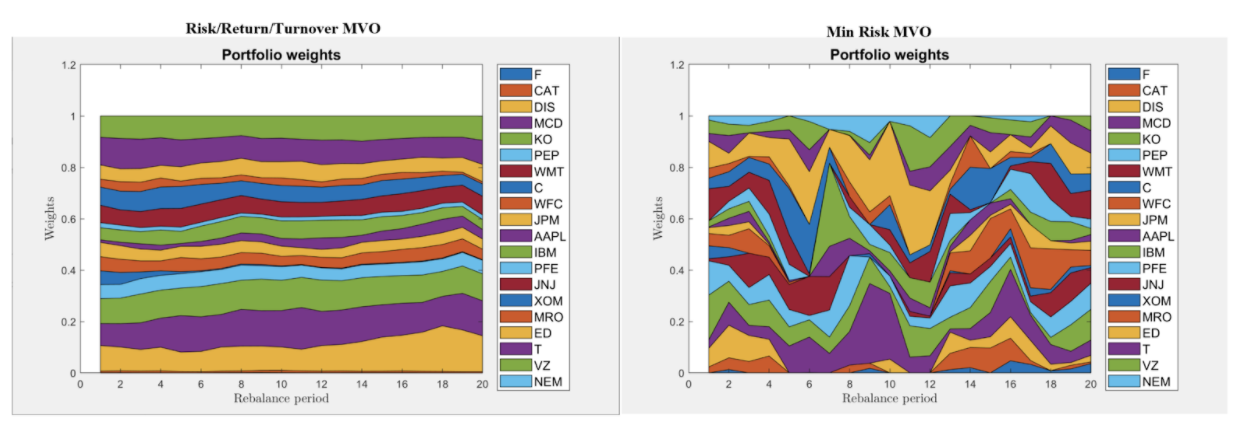
\includegraphics[scale=0.7]{pics/picture1.png}
    \caption{Contrast in Portfolio Weights for a stable (L) vs Unstable (R) model}
  \end{center}
\end{figure}

As can be seen in the figure above, the weighting remains stable once the penalty for asset turnover is added.  This is in contrast to \hyperref[sec:modelA]{\color{blue}Model A}, which does not account for transaction costs. The main reason why  two of the top three models performed better than the rest is because they took into account transaction costs.


\subsection{Second Round Analysis}
From the previous set of seven models, the aforementioned three models were chosen to perform a second, and final, round of further analysis, in order to determine an appropriate final model. The final round consisted of investigating the impact of various factor models, adjusting the exposure limits and short selling abilities, and varying $\lambda$. Results of each of these aspects of analysis are given in the following sections.  
\subsubsection{OLS}
To begin, three different versions of factor models were applied to the best three models, that is Models \hyperref[sec:modelD]{\color{blue}D}, \hyperref[sec:modelF]{\color{blue}F}, and \hyperref[sec:modelG]{\color{blue}G} in order to further determine which was optimal. The chosen factor models were the \hyperref[sec:ffff]{\color{blue}Five-Factor Fama-French} model, the \hyperref[sec:three]{\color{blue}Combination of Three Factors}, and the basic \hyperref[sec:ols]{\color{blue}OLS}. The \hyperref[sec:capm]{\color{blue}CAPM} model was considered, but not included, as it resulted in outcomes that were very similar, if not worse, than the Five Factor Fama-French model.\bigskip

It shall also be noted that analysis was done for two different time horizons; one for three years, as can be seen in Table 3 and one for one year, as can be seen in Table 4. The reasoning for analyzing different time horizons was due to the precision vs accuracy tradeoff. Including a longer timeframe for data would have led to an increased quantity of historical data, however, a longer timeframe has a higher probability of being less relevant. Therefore, both options were explored and analyzed to determine the optimal time frame alongside the optimal factor model. The following table shows the results of applying each factor model to the top three choices for final models, in a three year horizon: \bigskip
\begin{table}[!htbp]
\footnotesize
\centering
\begin{tabular}{c | c c | c c  | c c } 
\hline 
\rule{0pt}{3ex}  \multirow{2}{*}{\textbf{Model}} & \multicolumn{2}{c|}{Basic OLS} & \multicolumn{2}{c|}{Five Factor Fama-French} & \multicolumn{2}{c}{Combination of Three Factors} \\[1ex]\cline{2-7} 
\rule{0pt}{3ex} &  Sharpe  &  Turnover &  Sharpe  &  Turnover & Sharpe  &  Turnover  \\[1ex]
\hline 
\rule{0pt}{3ex}Model D        & 
0.1679 &  0.0087 & 0.1821 & 0.0059 & 0.1796  & 0.0060 \\ [1ex]
Model F   &0.1806 & 0.3281 & 0.1765 & 0.3349 & 0.1669 & 0.2532          \\ [1ex]
Model G   & 0.1922 &   0.0018 & 0.1819 & 0.0009  & 0.1877 & 0.0006     \\ [1ex]
\hline
\end{tabular}
\caption{Different Factor Models for a Three-Year Horizon}
\label{table:results}
\end{table}
From the Table 3, it was found that while using the baseline OLS regression, the best Sharpe Ratio was found with Model G: Robust Risk-Return with Ellipsoidal Uncertainty Set and Asset Turnover Tradeoff.  This is likely since this model includes/combines the objective function of the other two models, albeit with further coefficients. Furthermore, Model G performed relatively similarly, if not better, than the other models, regardless of  which factor model was used.  \bigskip

The following table compares the three optimization models with the three regression models using one year of historical data:\bigskip
\begin{table}[!htbp]
\footnotesize
\centering
\begin{tabular}{c | c c | c c  | c c } 
\hline 
\rule{0pt}{3ex}  \multirow{2}{*}{\textbf{Model}} & \multicolumn{2}{c|}{Basic OLS} & \multicolumn{2}{c|}{Five Factor Fama-French} & \multicolumn{2}{c}{Combination of Three Factors} \\[1ex]\cline{2-7} 
\rule{0pt}{3ex} &  Sharpe  &  Turnover &  Sharpe  &  Turnover & Sharpe  &  Turnover  \\[1ex]
\hline 
\rule{0pt}{3ex}Model D   & 0.1901&0.0303&0.1993&0.0329&0.1871&0.0264 \\ [1ex]
Model F   & 0.2323&0.9159&0.2131&0.9112&0.2197&0.7452\\ [1ex]
Model G   &0.1861&0.0005&0.1930&0.0005&0.1891&0.0010 \\ [1ex]
\hline
\end{tabular}
\caption{Different Factor Models for a One-Year Horizon}
\label{table:results}
\end{table}

The general trend was that the Sharpe Ratio increased using only one year of historical data, but the asset turnover also increased. This is because as the market changes, the expected returns in the model are able to adapt to these changes faster because they use more relevant/recent market data compared to the three year time horizon. In addition, the asset turnovers, in general, increase because the expected returns were more dynamic. This causes the regression of each asset to fluctuate more and causes the model to update the model weights faster in response to the faster changes in the regression.\bigskip

To conclude, the Five Factor Fama-French model using one year of historical data provided the best Sharpe Ratio and lowest asset turnover for Model G. 
\subsubsection{Short Selling and Exposure Limits}
After converging to the one year, Five Factor Fama-French model with Model G,  the short selling/exposure limits can be adjusted to maximize returns, while making sure too much weight is not given to a single asset or over leverage the portfolio. The table below summarizes different exposure limits and resulting Sharpe Ratio and Asset Turnover Rate. Let $L_i$ and $U_i$ be the minimum and maximum weight of each asset, respectively.\bigskip

\begin{table}[!htbp]
\footnotesize
\centering
\begin{tabular}{c |c c c c c | c c} 
\hline
\rule{0pt}{3ex}  \multirow{2}{*}{\textbf{Model}} & \multicolumn{5}{c|}{$L_i =$ [ ]} & \multicolumn{2}{c}{$L_i = 0$}  \\[1ex]\cline{2-8} 
\rule{0pt}{3ex} &  $U_i = 0.2$  &  $U_i = 0.25$ &  $U_i = 0.3$  &  $U_i = 0.35$ & $U_i = 1$  &  $U_i = 0.3$ & $U_i = 1$ \\[1ex]
\hline
\rule{0pt}{3ex}Sharpe Ratio & 0.1814 & 0.1919 & 0.1935 & 0.1873& 0.1877 & 0.1897 & 0.1893
  \\ [1ex]
Asset Turnover     & \num{6.1e-05}& \num{3.0e-0.7}& \num{3.5e-08}
&\num{2.8e-08} & \num{2.2e-08} & \num{1.2e-03} & \num{1.1e-03}
        \\ [1ex]
\hline
\end{tabular}
\caption{Fine Tuning of Exposure Limits and Short Selling on Model G}
\label{table:results}
\end{table}
The best exposure parameters for the model were to have no lower bound, therefore allowing short selling, and an upper bound of 0.35 on each asset. \bigskip

Shorting allows the model to sell assets that have low expected returns so that the model can invest more capital in assets predicted to have higher returns. One pitfall with allowing short selling is that the model could very easily become over leveraged, shorting positions with a large weight of capital to over 100\% of the capital and going long with over 100\% of the capital to balance this out. The risk of this could have been reduced by putting a lower bound of $-n$\% for each asset, however, the robust model takes into account uncertainty within the expected return parameter to reduce the risk of over leveraging, thus reducing the need for the lower bound to be set. \bigskip

In addition, there is no real benefit of narrowing down the upper bound more than the 35\%, as the returns would likely be the result of overfitting the data set. Considerations to avoid overfitting were made due to the fact that when new, unseen data is used in the model, results would be suboptimal if the model had been overfit to the sample data.  
\subsubsection{Adjusting Lambdas}
The model has three $\lambda$ parameters to weight the variance ($\lambda_1$), expected return ($\lambda_2$), and the turnover ratio ($\lambda_3$). \bigskip

\begin{table}[!htbp]
\footnotesize
\centering
\begin{tabular}{c |c |c |c |c |c |c} 
\hline
\rule{0pt}{3ex}  \multirow{3}{*}{}  & $\lambda_1 = 1$ & $\lambda_1 = 1$ & $\lambda_1 = 1$ & $\lambda_1 = 5$ & $\lambda_1 = 20$ & $\lambda_1 = 40$   \\[1ex]
\rule{0pt}{3ex} & $\lambda_2 = 1$ & $\lambda_2 = 5$ & $\lambda_2 = 1$ & $\lambda_2 = 1$  & $\lambda_2 = 1$  & $\lambda_2 = 1$  \\[1ex]
\rule{0pt}{3ex} & $\lambda_3 = 1$ & $\lambda_3 = 1$ & $\lambda_3 = 0.1$ & $\lambda_3 = 0.5$  & $\lambda_3 = 0.5$ & $\lambda_3 = 0.5$   \\[1ex]
\hline
\rule{0pt}{3ex}Sharpe Ratio & 0.1867 & 0.1734 & 1845 & 0.1851& 0.1935 & 0.1892 
  \\ [1ex]
Asset Turnover     
&\num{9.7e-09} & \num{5.9e-05} & \num{5.2e-04} & \num{1.8e-08}& \num{3.5e-0.8}& \num{4.4e-07}
        \\ [1ex]
\hline
\end{tabular}
\caption{Fine Tuning of Lambdas for Optimal Performance on Model G}
\label{table:results}
\end{table}
Note that some steps towards the convergence of the lambdas were omitted. The final result was a weighting of $\lambda_1=20$ on the variance, $\lambda_2=1$ on the returns, and $\lambda_3=0.5$ on the asset turnover. \bigskip

One trend is that the Sharpe Ratio did not increase as the weighting on the expected returns increased. This could be due to the uncertainty around the returns parameter or that the variance increased at a faster rate than returns increased. As a result, the final weighting had a larger emphasis on the volatility relative to the expected returns. \bigskip

Another trend is that as the turnover factor decreased, the asset turnover increased. However, the Sharpe Ratio did not increase as the turnover factor decreased even though there was more weighting on the Sharpe Ratio in the objective function. This could be due to a few different reasons. Firstly, many assets in the portfolio had similar returns and switching them out each period, thereby increasing the turnover, did not improve the Sharpe Ratio because there is an abundance of uncertainty around the returns.\pagebreak
\section{Final Model Recommendation and Conclusion}
\hrule \vspace{15pt}
To conclude, the final model developed was a Robust Risk-Return model with an Ellipsoidal Uncertainty Set and included an Asset Turnover Tradeoff. After the first round of analysis and convergence to this model, the second round of parameter tuning was completed to determine the optimal Factor Model, exposure limits, and $\lambda$ values. \bigskip

Final results consisted of leveraging a Five Factor Fama-French model, with a one year time horizon, which would be applied to the final model. Furthermore, the exposure limits were chosen to have no lower bound on the asset weights, thereby allowing short selling, and implementing an upper bound of 0.35 for each asset. Finally, the objective function for the final model aims to; minimize risk, with $\lambda_1 =20$; maximize returns, with a $\lambda_2=1$; and minimize asset turnover, with $\lambda_3=0.5$.  The final model is given as: 
\[
\begin{aligned}
&\begin{aligned}
    & \min_{\bm{x}}     &&20 \bm{x}^T \bm{Q}\ \bm{x} - 1(\bm{\mu}^T \bm{x}  - \epsilon || \bm{\Theta}^{1/2}\bm{x} ||_2) + 0.5\bm{1}^T |\bm{x_0} - \bm{x}|
\end{aligned} \\
&\begin{aligned}
    &\ \mathrm{s.t.}        & \bm{1}^T \bm{x} &= 1 \\
    &                   & \bm{x} &\in \bm{\mathbb{R}}
\end{aligned}
\end{aligned}
\]
The results of the final model are promising and have not been overfit to the sample data, thereby allowing for optimal performance when new, unseen data is used. Output graphs of the Portfolio Weights (Figure 2) and Portfolio Wealth Evolution (Figure 3) can be seen below:
\begin{figure}[H]
    \centering
    \subfloat{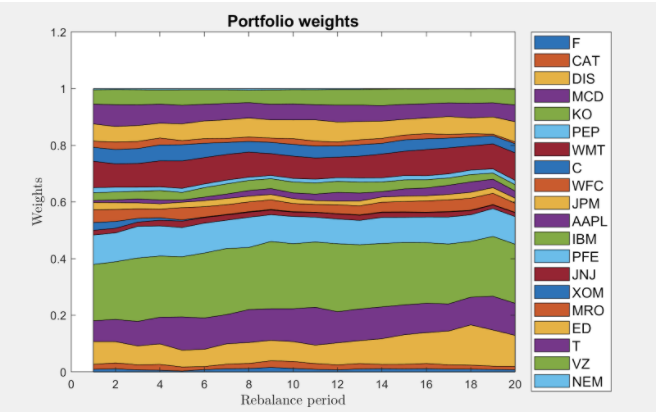
\includegraphics[scale=0.6]{pics/picture2.png}}%
    \qquad
    \subfloat{ 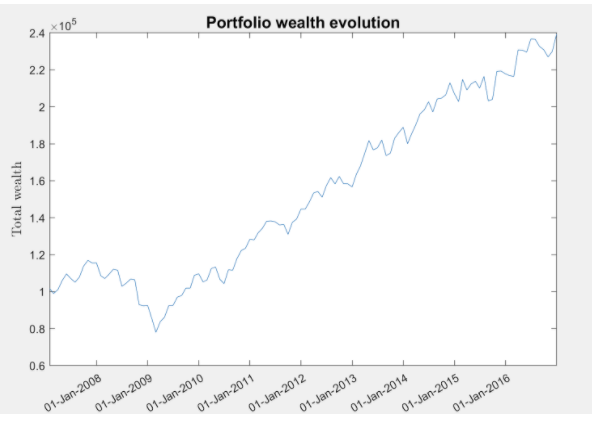
\includegraphics[scale=0.6]{pics/picture3.png} }%
    \caption{Final Model Portfolio Weights (L) and Wealth Evolution (R)}
\end{figure}


The portfolio weights are nicely balanced and smooth, while the portfolio wealth evolves from \$1,000,000 to \$2,400,000 over the time frame. This results in a CAGR of over 9\%, which is quite strong considering the time frame spans the Great Recession.\bigskip

Overall, the two-step analysis process allowed for convergence on a very strong final model, with optimal results. 



\end{document}


